\section*{Exercise 1}
In this assignment, we implement the k-means algorithm for clustering the input data points.
Clustering is considered as a unsupervised machine learning problem, that means there no labels in the data that we need to predict as classification, but it helps us getting some insights about the input data.

We developed four methods for initializing the first K cluster centroids (where K is an input)
The first one is just choosing the first K data points to be the centroids, the second method is randomized selections of the initial centroids. the third method is k-means++
and the fourth method is using Gonzales’ algorithm.

For each method, we run k-means for different values of k {3,4,5} and in randomized methods, we run that 5 times. we visualise the results to get more understanding and learning experience as shown below.



\begin{figure}[!h]
\centering
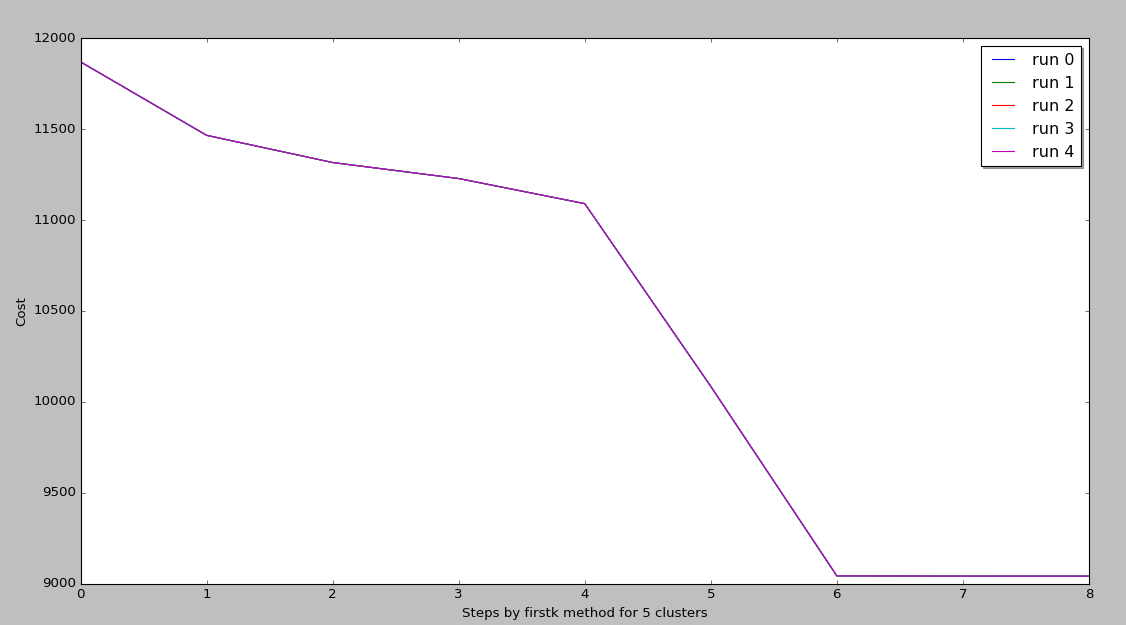
\includegraphics[width=0.9\textwidth]{shots/firstk5clusters.png}
\caption{ }
\label{barcharthover}
\end{figure}







